\documentclass[letterpaper, landscape]{exam}
\usepackage{2in1, lscape} 
\printanswers

\usepackage{units} 
\usepackage[fleqn]{amsmath}
\usepackage{float}
\usepackage{mdwlist}
\usepackage{booktabs}
\usepackage{caption}
\usepackage{fullpage}
\usepackage{enumerate}
\usepackage{graphicx}

\setcounter{tocdepth}{1}
\everymath{\displaystyle}

\author{}
\date{\today}
\title{Calculus I \\ Week Five}

\begin{document}

  \maketitle
  \tableofcontents

  \section{Homework Three} 
  \begin{itemize}
    \item TO DO
  \end{itemize}

  \section{Continuity Definition}

  A function is continuous at $a$ if:
  \[
    \lim_{x \to a} f(x) = f(a) 
  \]

  \begin{itemize*}
    \item implies $\lim_{x \to a} f(x)$ is defined
    \item implies $f(a)$ is defined
    \item matches intuitive idea for continuous line
    \item can draw graph without lifting pen from paper
    \item draw examples of continuous and discontinuous functions including:
      \begin{itemize*}
        \item $f(x)$ undefined at $a$
        \item hole at $f(a)$ with $f(a)$ defined at a different value
        \item left limit not equal to right limit
      \end{itemize*}

    \item a {\em removable} discontinuity occurs when $f(x)$ is undefined at $a$. It can
      be removed by defining a suitable value for $f(a)$.

  \end{itemize*}

  examples:
  \begin{enumerate}
    \item 
      \[
        f(x) = \frac{1}{x - 1}
      \]
      
      $f(1)$ doesn't exist and $\lim_{x \to 1} f(x)$ also doesn't exist (See Figure
      \ref{fig:ex01}).

      \begin{figure}[H]
        \centering
        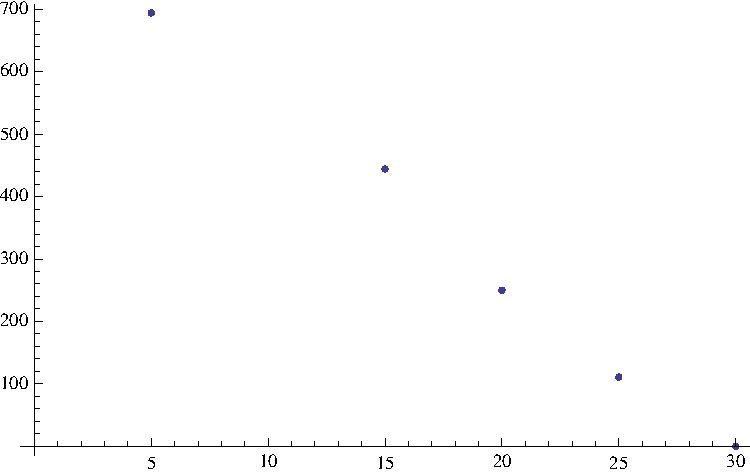
\includegraphics[scale = 0.5]{ex01.pdf}
        \caption{Example 1}
        \label{fig:ex01}
      \end{figure}

    \item 
      \[
        f(x) = \frac{x^2 - 1}{x - 1} = x + 1
      \]
      
      $f(1)$ doesn't exist. This is an example of a {\em removable discontinuity}

    \item
        \[
          f(x) = 
            \begin{cases}
              \frac{x^2 - 1}{x - 1} & \text{if } x \neq 1 \\
              0                     & \text{if } x = 1 \\
            \end{cases}
        \]

        $f(1) \neq\lim_{x \to 1} f(x)$

    \item
        \[
          f(x) = 
            \begin{cases}
              \frac{x^2 - 1}{x - 1} & \text{if } x \neq 1 \\
              2                     & \text{if } x = 1 \\
            \end{cases}
        \]

        continuous

  \end{enumerate}

  \section{Left and Right Continuity}
  
  \begin{description}
    \item[Continuous from the Left] $\lim_{x \to a-} f(x) = f(a)$ 
    \item[Continuous from the Right] $\lim_{x \to a+} f(x) = f(a)$ 
  \end{description}

  \section{Continuous on an Interval}
  A function is continuous on an interval if it is continuous at every point in the
  interval.

  \section{Combining Continuous Functions}
  If $f$ and $g$ are continuous at $a$ and $c$ is a constant, all of these are also
  continuous:

  \begin{itemize}
    \item $f \pm g$
    \item $fg$
    \item $\frac{f}{g}$ if $f(a) \neq 0$
    \item $cf$
  \end{itemize}

\end{document}

